%!TEX root = ../../main.tex
\toggletrue{image}
\toggletrue{imagehover}
\chapterimage{form}
\chapterimagetitle{\uppercase{Form}}
\chapterimageurl{https://xkcd.com/608/}
\chapterimagehover{'This space intentionally left blank' is less immediately provocative but more Hofstadterially confusing.}

\chapter{Formulare mit \ac{PHP} verarbeiten}
\label{chapter-formulare-php}

\begin{wrapfigure}[12]{r}{7cm}
\vspace{-\baselineskip}
\centering
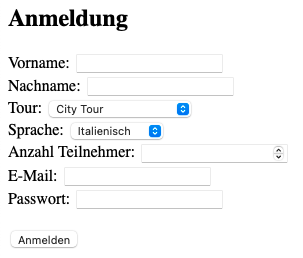
\includegraphics[scale=0.55]{anmeldung}
\caption{Formular mit \lstinline{input}- und \lstinline{select}-Elementen.}
\label{figure-anmeldung}
\end{wrapfigure}

Sie kennen vermutlich Webseiten, auf denen Sie aufgefordert werden, in bestimmten Feldern etwas einzugeben. Beim Online-Shopping wird nach der Adresse gefragt, bei einem Newsletter muss man die E-Mail-Adresse angeben oder beim Log-in wird der Benutzername und das Passwort abgefragt. \autoref{figure-anmeldung} zeigt ein Beispiel. Solche Webseiten können mit einem \ac{HTML}-Formular (eng. form) realisiert werden. \ac{PHP} übernimmt die Aufgabe, die Formulardaten zu verarbeiten. Ein \ac{HTML}-Formular in Kombination mit \ac{PHP} ist der praktikabelste Weg, Ihre Webseite interaktiv zu machen. Die Lernziele von diesem Kapitel lauten:

\newcommand{\formulareMitPhpVerarbeitenLernziele}{
\protect\begin{todolist}
\item Sie verarbeiten Formulardaten mit \ac{PHP}.
\end{todolist}
}

\lernziel{\autoref{chapter-formulare-php}, \nameref{chapter-formulare-php}}{\protect\formulareMitPhpVerarbeitenLernziele}

\formulareMitPhpVerarbeitenLernziele

\section{\ac{HTML}-Formulare}

Das \lstinline{<form>}-Element besitzt zwei Attribute, um die Verarbeitung der Formulardaten zu konfigurieren. Das \lstinline{action}-Attribut bestimmt, welche Webseite nach dem Klicken auf den \say{submit}-Button aufgerufen wird. Das \lstinline{method}-Attribut definiert die Übertragungsmethode. Der Standardwert lautet \lstinline{get} (Datenübertragung via \ac{URL}). Alternativ können wir \lstinline{post} verwenden. Dann werden die Daten im \say{Hintergrund} übertragen. Dies bedeutet \textbf{nicht}, dass die Daten verschlüsselt übertragen werden! \autoref{lst-form-action} zeigt ein Beispiel mit einer \ac{PHP}-Datei und \texttt{post}.

\begin{lstlisting}[language=HTML, caption={Wenn wir auf den Button klicken, dann wird die Datei \texttt{feedback.php} aufgerufen.}, label={lst-form-action}]
<form action="feedback.php" method="post">
 <label for="vorname">Vorname:</label>
 <input type="text" id="vorname" name="vorname" required>
 <label for="nachname">Nachname:</label>
 <input type="text" id="nachname" name="nachname" required>
 <button type="submit" name="anmelden">Anmelden</button>
</form>
\end{lstlisting}

In der \say{action}-Datei stehen dann die Formulardaten zur Verarbeitung zur Verfügung. Wir verwenden als \say{action}-Datei immer eine \ac{PHP}-Datei, damit wir die Formulardaten in einem \ac{PHP}-Abschnitt verarbeiten können.

\section{Formulardaten verarbeiten}

Wir besprechen nun die Datenverarbeitung für beide Methoden (\texttt{POST}-Methode und \texttt{GET}-Methode). Die Datenverarbeitung läuft für beide Methoden sehr ähnlich. Wir zeigen zunächst die Verarbeitung mit der \texttt{POST}-Methode und sprechen dann die Unterschiede bei der \texttt{GET}-Methode an.

\subsection{\texttt{POST}-Methode}

In der \say{action}-Datei stehen mit der globalen Variablen \lstinline{$_POST} die Formulardaten zur Verfügung, falls wir beim \lstinline{method}-Attribut den Wert \lstinline{post} angeben. Mit \lstinline{$_POST} können wir auf die einzelnen \lstinline{input}- und \lstinline{select}-Elemente eines Formulars zugreifen. Dabei müssen wir in den eckigen Klammern den Namen des Formularelements notieren. Möchten wir etwa den Vornamen auslesen, dann müssen wir \lstinline{$_POST["vorname"]} verwenden. Der String in den eckigen Klammern muss identisch sein mit dem Wert des \lstinline{name}-Attributs. In \autoref{lst-form-action} ist dies zum Beispiel \lstinline{name="vorname"}. Gross- und Kleinschreibung ist dabei strikt zu beachten. \autoref{lst-read-form-data-post} zeigt ein Beispiel.

\begin{lstlisting}[language=PHP, alsolanguage=HTML, caption={Daten können direkt ausgeben oder zuvor in einer Variablen gespeichert werden.}, label={lst-read-form-data-post}]
<!DOCTYPE html>
<html lang="de">
<head>
 <meta charset="UTF-8"><title>Feedback</title>
</head>
<body>
  <h2>Danke fuer Ihre Anmeldung</h2>
  <ul>
    <li>Vorname: <?php echo $_POST["vorname"]; ?></li>
    <li>Nachname: 
      <?php 
      $eingabe_nachname = $_POST["nachname"]; 
      echo $eingabe_nachname; 
      ?>
    </li>
  </ul>
</body>
</html>
\end{lstlisting}

\subsection{\texttt{GET}-Methode}

Die Datenverarbeitung erfolgt nun über die globale Variable \lstinline{$_GET}, falls wir beim \lstinline{method}-Attribut den Wert \lstinline{get} angeben. Ansonsten ändert sich bei der Datenverarbeitung nichts. \autoref{lst-read-form-data-post} zeigt den geänderten Code im Vergleich zu \autoref{lst-read-form-data-get}.

\begin{lstlisting}[language=PHP, alsolanguage=HTML, caption={Die globale Variable \lstinline{$_GET} muss bei \lstinline{method="get"} benutzt werden.}, label={lst-read-form-data-get}]
<li>Vorname: <?php echo $_GET["vorname"] ?></li>
<li>Nachname: 
  <?php 
  $eingabe_nachname = $_GET["nachname"]; 
  echo $eingabe_nachname; 
  ?>
</li>
\end{lstlisting}